\documentclass[a4paper,12pt]{article} % This defines the style of your paper

\usepackage[top = 2.5cm, bottom = 2.5cm, left = 2.5cm, right = 2.5cm]{geometry} 

\usepackage[T2A]{fontenc}
\usepackage[utf8]{inputenc}
\usepackage[russian]{babel}

\usepackage{multirow} 
\usepackage{booktabs} 

\usepackage{graphicx} 
\graphicspath{}

\usepackage{setspace}
\setlength{\parindent}{0in}

\usepackage{float}

\usepackage{amsmath}

\usepackage{fancyhdr}

\usepackage{pgfplots}

\pgfplotsset{compat=1.9}

\pagestyle{fancy} 

\fancyhf{} 

\lhead{\footnotesize Расчетное задание №12}

\rhead{\footnotesize Николаев Юрий} 

\cfoot{\footnotesize \thepage} 

\begin{document}

\thispagestyle{empty} 

\begin{tabular}{p{15.5cm}} 
НИУ МЭИ \\ А-13а-19  \\ Вариант 13 \\ Николаев Юрий\\
\hline 
\\
\end{tabular} 

\vspace*{0.3cm}

\begin{center} 
	{\Large \bf Расчетное задание №12} 
	\vspace{2mm}
\end{center}  

\vspace{0.4cm}


\section{Задание}
Выполнить три итерации по методу Зейделя для системы уравнений $Ax = b$ (не переставляя строк). В качестве начального приближения взять нулевой вектор. Изобразить графически поведение итерационного процесса. Сопоставить наблюдаемое поведение метода с выполнением достаточных условий сходимости метода.

\begin{center}
\begin{tabular}{ | c c | c | }
\hline
 \multicolumn{2}{| c |}{A} & b \\ \hline 
3 & 3 & 3 \\
4 & 3 & 3 \\

\hline
\end{tabular}
\end{center}

\section{Решение}

\begin{enumerate}

\item Преобразование Якоби и расчетные формулы метода.

\begin{equation*}
\begin{cases}
    x_1^{(n+1)} = \frac{1}{3}(-3x_2^{(n)} + 3) \\
    x_2^{(n+1)} = \frac{1}{3}(-4x_1^{(n+1)} + 3) \\
\end{cases}
\end{equation*}

\begin{center}
\begin{tabular}{| c | c  c |}
\hline
    n & $x_1^{(n)}$ & $x_2^{(n)}$ \\ \hline
    0 & 0 & 0  \\
    1 & 1 & -1/3 \\
    2 & 4/3 & -7/9 \\
    3 & 16/9 & -37/27 \\
\hline
\end{tabular}
\end{center}

\begin{equation*}
    B =
    \begin{pmatrix}
        0 & -1 \\
        -\frac{4}{3} & 0  \\
    \end{pmatrix}
\end{equation*}

Проверим необходимое условие сходимости метода Зейделя:

$\|B_1\| + \|B_2\| = 1 + 4/3 = 5/3 > 1$ - условие не выполняется.

\vspace{0.4cm}

По графику (Рис. 1) видно, что каждая итерация идет в противоположную сторону от решения СЛАУ. Это сопостовимо тому, что необходимое условие сходимости метода Зейделя не выполняется.

\begin{figure}[h]
\center{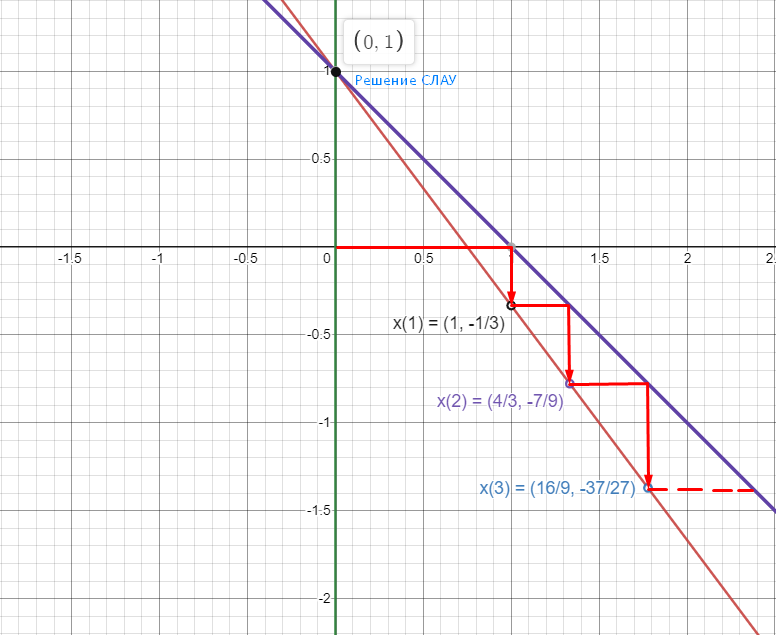
\includegraphics[scale=0.6]{rz_12.png}}
\caption{График с итерациями}
\label{fig:image}
\end{figure}

\newpage

\item Найдем собственные числа матрицы $B$, увидим, что условие сходимсоти не выполнено, так как все собственные числа данной матрицы по модулю больше единицы.

\begin{pmatrix}
        -\lambda & -1 \\
        -\frac{4}{3} & -\lambda  \\
    \end{pmatrix}
    
$\lambda^2 = \frac{4}{3} \Rightarrow |\lambda| = |\pm \sqrt{\frac{4}{3}}| \approx 1,15 > 1$



\end{enumerate}

\end{document}